\section{Experimental results}
\label{exper}

\subsection{Model accuracy}

We observe from table \ref{tbl:results} that performance improved significantly as we increase the percentage of labeled data for all models. Of the four models, the supervised baseline model observed the largest boost in model performance of 30\% from when we increased from 1\% to 10\% labels. Whereas, our SimCLR framework observed the smallest increase in prediction accuracy of around 5\%. Further, we observe that SimCLR with linear evaluations outperforms the baseline model by 15\% on 1\% labeled data, but the baseline model performs better on 10\% labeled data. 
In other words, SimCLR achieves a much better performance on almost no labels to train on but benefits less from more data labels in our implementation.

In comparison to all other models, RotNet performs the worst when linearly evaluated. It achieves a lower test accuracy than our baseline model at 1\% and SimCLR model at 10\%. This was expected as the RotNet ConvNet representations were not intended, according to the paper \cite{RotNet}, to be used in a linear manner downstream. Instead, the framework expects continued training with limited labeled data to be evaluated in its semi-supervised state. In our implementation, our semi-supervised RotNet model achieved the best model accuracy of 70.71\% with only 1\% data labels and 83.64\% with 10\%.


% Insert table of evaluation results
\begin{table}[!htbp]
    \centering
    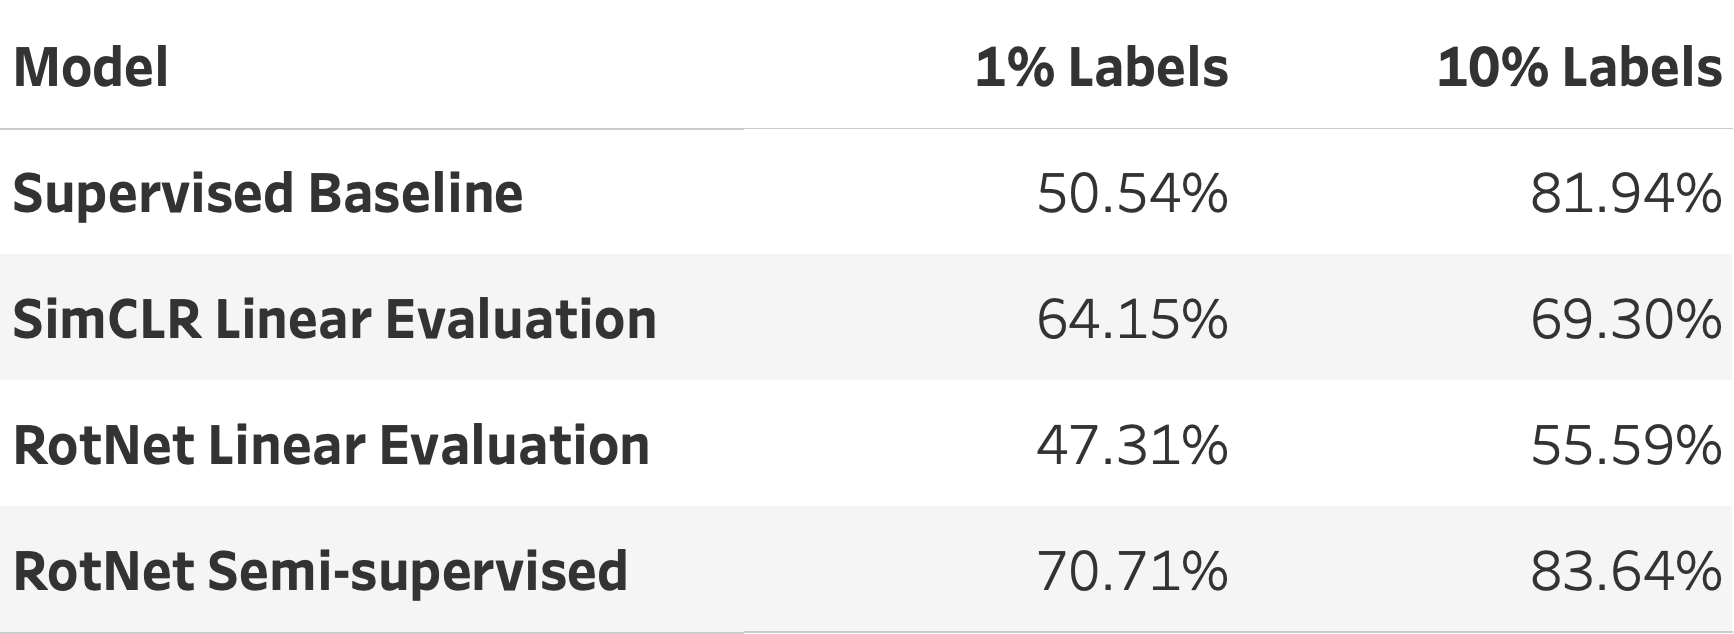
\includegraphics[width=.60\linewidth]{figs/results}
    \vspace{0.2cm}
    \caption{Model performance on 1\% and 10\% labeled data}
    \label{tbl:results}
\end{table}

Overall, the results from our implementations are within reasonable range as compared to the two papers \cite{SimCLR} \cite{RotNet}. Our RotNet achieved results on par with the paper while our SimCLR implementation achieved lower accuracy than that from the paper on CIFAR-10. We believe variation in model performance could be due the different encoder model and our limited resources to fine-tune our hyper-parameters and run for longer epochs.

\subsection{Discussion}

From the linear evaluation experiments performed on both the SimCLR and the RotNet, we observe that SimCLR performs significantly better than the RotNet. A potential implication of this could be that the representations learned by the encoder of the SimCLR are readily applicable to downstream tasks like image classification. Whereas the RotNet would require additional fine-tuning of the last residual block (i.e. its semi-supervised setting) to increase model performance.

We visualize the representations learned at the end of each block of our ResNet-20 model from our supervised, SimCLR, and RotNet in Figure \ref{featmap} to gain insight on our results.

% Insert images of representations learned
\begin{figure}

\centering
\subfloat[Baseline Block 1]{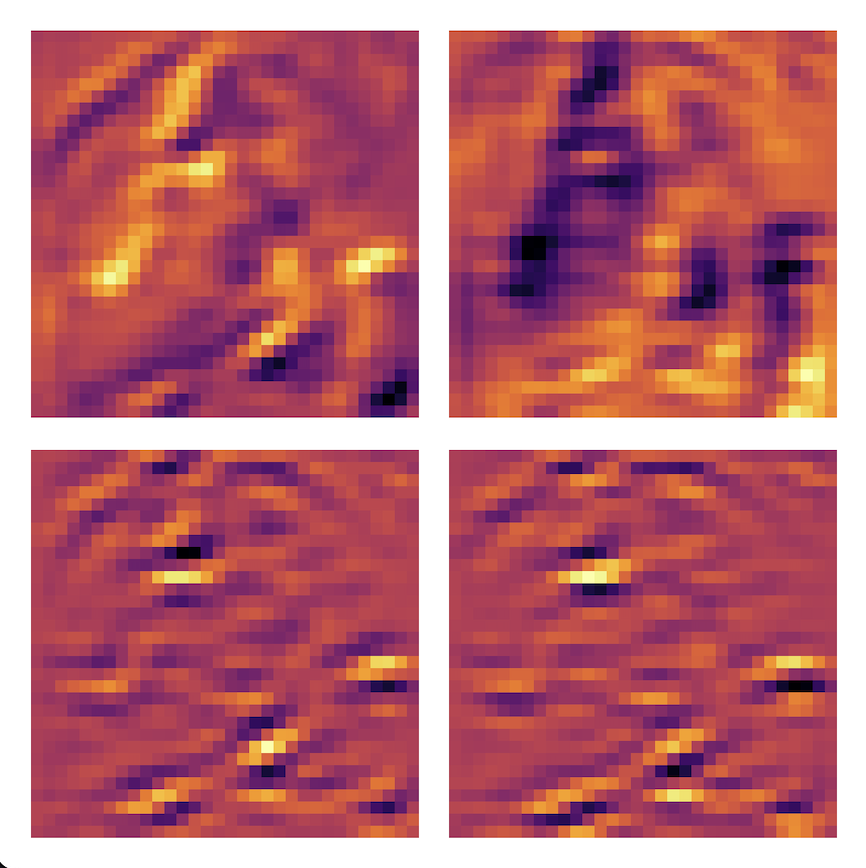
\includegraphics[width=0.3\linewidth]{figs/BaseRep1.png}}\hfil
\subfloat[SimCLR Block 1]{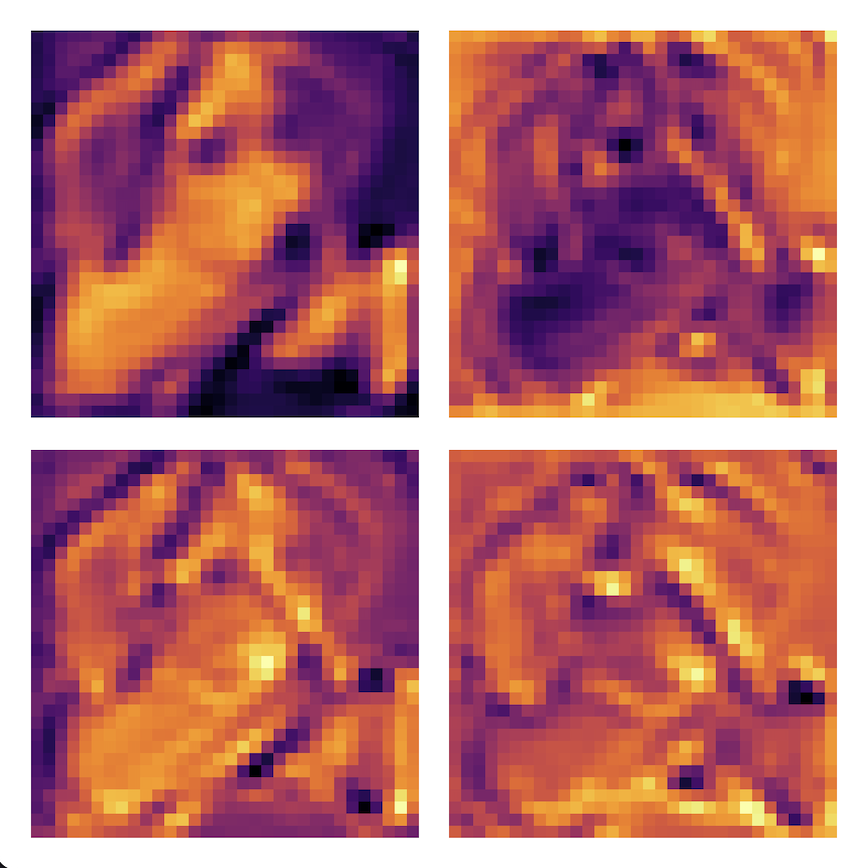
\includegraphics[width=0.3\linewidth]{figs/SimRep1.png}}\hfil
\subfloat[RotNet Block 1]{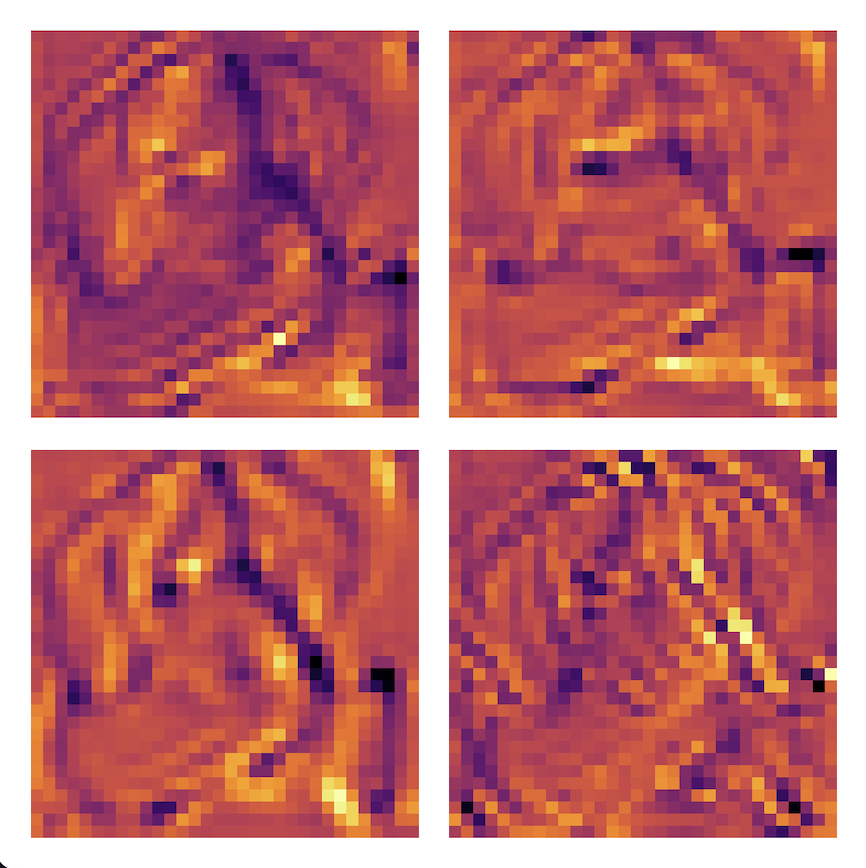
\includegraphics[width=0.3\linewidth]{figs/RotRep1.png}}

\subfloat[Baseline Block 2]{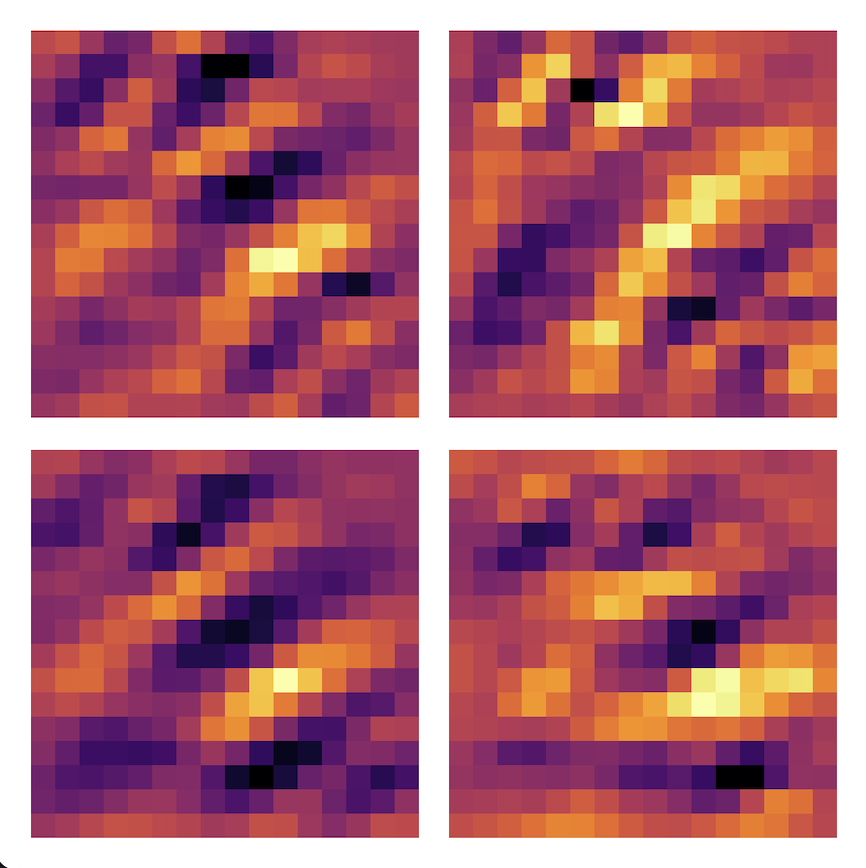
\includegraphics[width=0.3\linewidth]{figs/BaseRep2.png}}\hfil 
\subfloat[SimCLR Block 2]{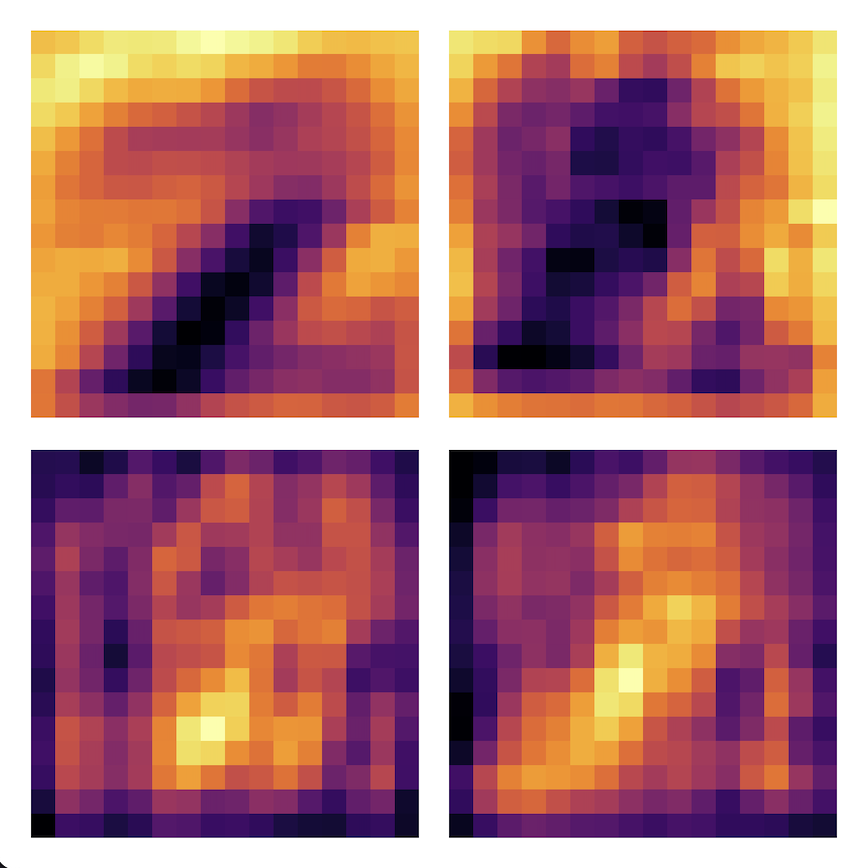
\includegraphics[width=0.3\linewidth]{figs/SimRep2.png}}\hfil
\subfloat[RotNet Block 2]{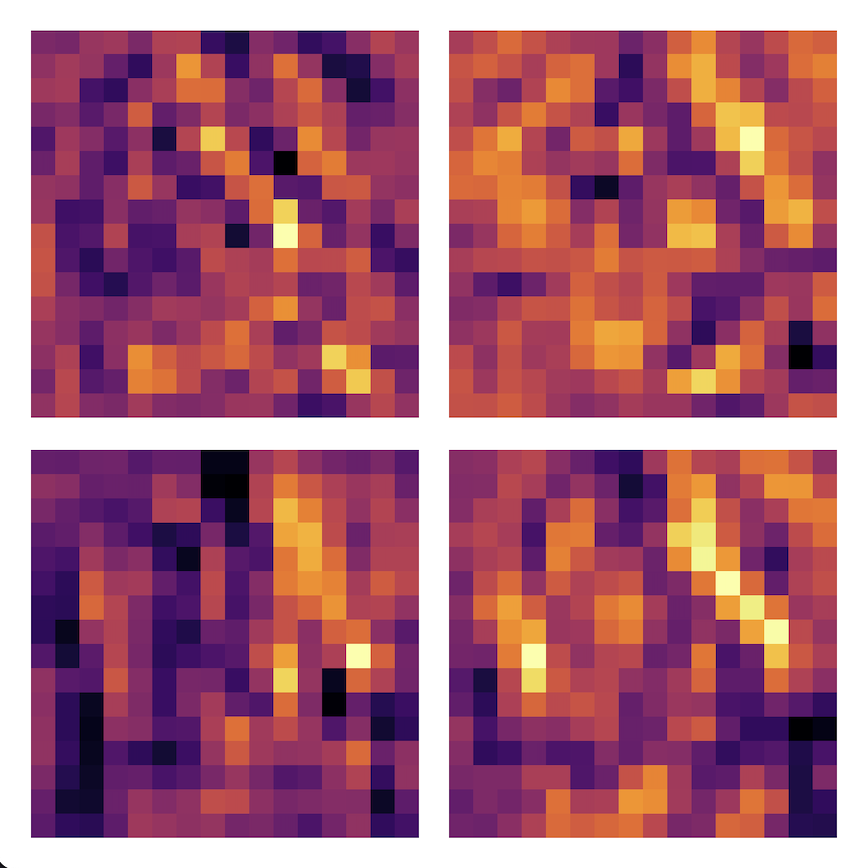
\includegraphics[width=0.3\linewidth]{figs/RotRep2.png}}

\subfloat[Baseline Block 3]{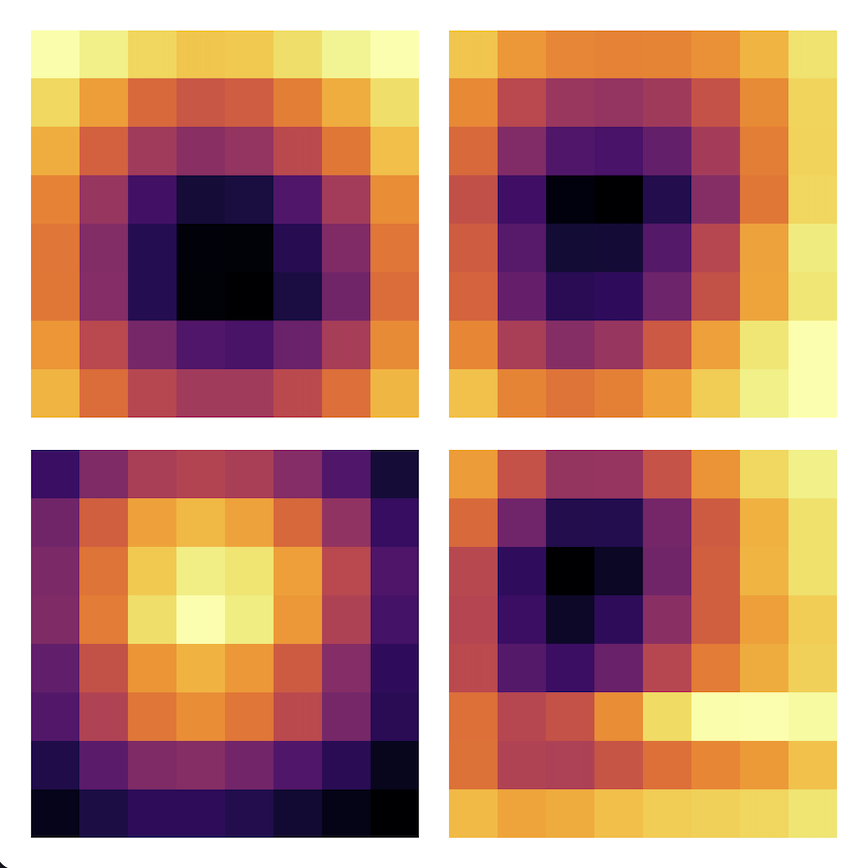
\includegraphics[width=0.3\linewidth]{figs/BaseRep3.png}}\hfil 
\subfloat[SimCLR Block 3]{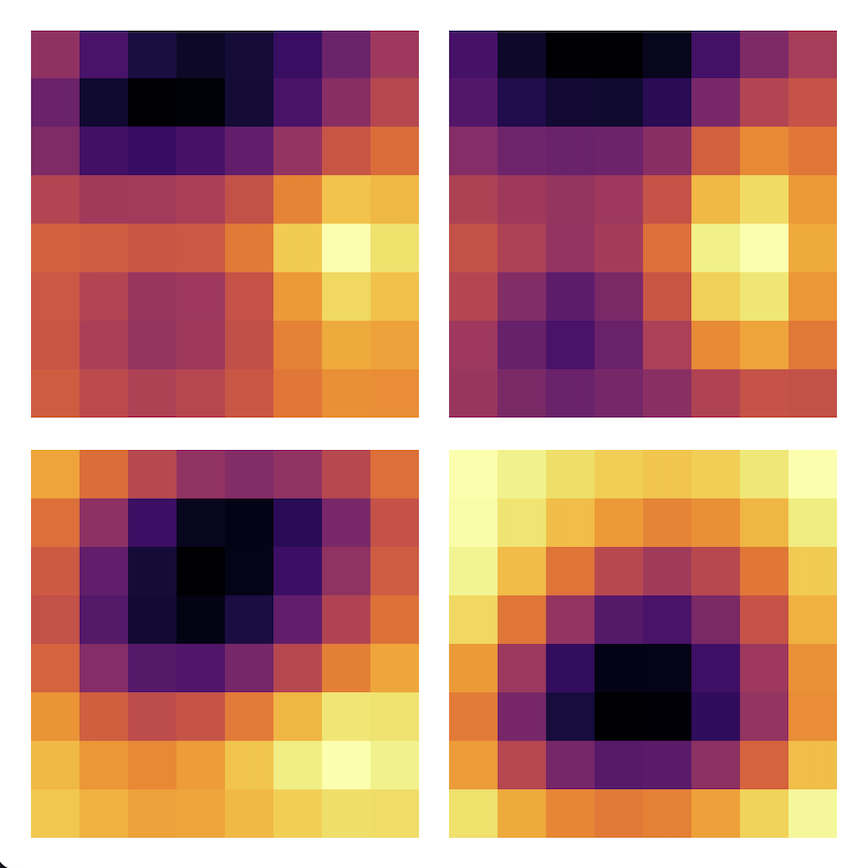
\includegraphics[width=0.3\linewidth]{figs/SimRep3.png}}\hfil
\subfloat[RotNet Block 3]{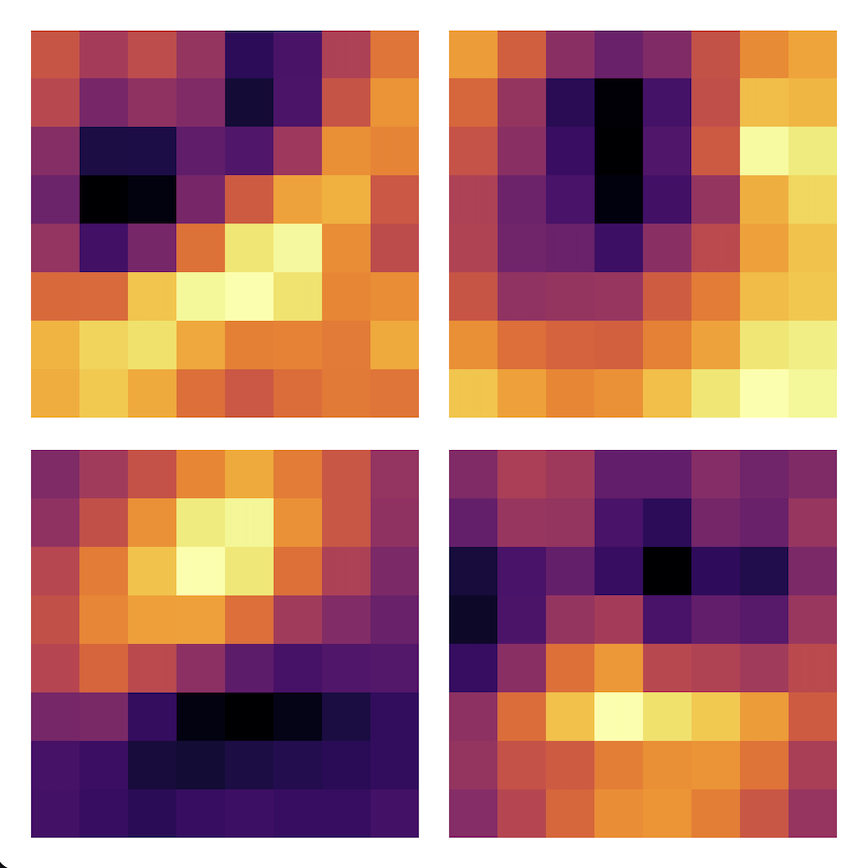
\includegraphics[width=0.3\linewidth]{figs/RotRep3.png}}

\caption{Feature maps from last layer of each ResNet-20 residual block (4 filters shown)}\label{featmap}
\end{figure}


If we look at the first blocks in Figure \ref{featmap}(a), (b), and (c), we observe the baseline model appear to learn a variety of different features, whereas SimCLR and RotNet appear to learn more targeted features. Specifically, the RotNet model seem to focus on learning outlines of objects. The difference between the types of features learned by SimCLR and RotNet could explain why SimCLR performs better than RotNet as a linear classifier for this particular dataset.

